\subsection{Buscas contínuas}
\begin{table}[!ht]\centering\caption{Modas de $f$ nas 100 rodadas por método}
\scriptsize\setlength{\tabcolsep}{4pt}\begin{tabular}{lrrrrr}\toprule
Função & Método & Passo & Acertos & Moda & Freq.\\
\midrule
Esfera & HC & $0{,}750$ & 94 & $0{,}00$ & 71\\
Esfera & LRS & $0{,}050$ & 6 & $0{,}00$ & 6\\
Esfera & GRS & --- & 0 & $5{,}00$ & 2\\
Gaussianas & HC & $0{,}750$ & 1 & $1{,}01$ & 52\\
Gaussianas & LRS & $0{,}010$ & 68 & $2{,}00$ & 68\\
Gaussianas & GRS & --- & 20 & $1{,}98,\;2{,}00$ & 16\\
Ackley & HC & $1{,}000$ & 0 & $0{,}10,\;0{,}15,\;0{,}22$ & 6\\
Ackley & LRS & $0{,}500$ & 2 & $0{,}15$ & 9\\
Ackley & GRS & --- & 0 & $2{,}61,\;3{,}20$ & 3\\
Rastrigin & HC & $1{,}000$ & 0 & $0{,}05,\;0{,}09,\;0{,}62,\;1{,}02$ & 3\\
Rastrigin & LRS & $0{,}500$ & 2 & $1{,}01$ & 4\\
Rastrigin & GRS & --- & 0 & $5{,}01$ & 3\\
Mista & HC & $0{,}010$ & 0 & $1{,}44$ & 100\\
Mista & LRS & $0{,}010$ & 12 & $2{,}00$ & 12\\
Mista & GRS & --- & 0 & $1{,}40$ & 5\\
\bottomrule\end{tabular}\end{table}
Na Esfera, o HC atingiu a tolerância em 94 rodadas com abertura 0,75. Nas Gaussianas, o HC aproximou o máximo em uma rodada, mas sua moda 1,01 indica concentração perto do pico local. Na Ackley e na Rastrigin, apenas a LRS atingiu a tolerância na grade testada. Na função mista, o HC ficou na fronteira inicial com abertura 0,01, e a LRS atingiu a tolerância em 12 rodadas. A escolha de passo pelo primeiro acerto favorece a menor abertura observada, mesmo quando a taxa de sucesso é baixa. As coordenadas finais e o erro mediano constam nos CSVs.
\subsection{Oito rainhas}
As 92 soluções apareceram em 1099 rodadas, com 1022 sucessos e 1005509 iterações em $3{,}47$ s. Houve 930 soluções repetidas e 77 rodadas sem sucesso. A primeira solução foi $(6, 4, 1, 5, 8, 2, 7, 3)$.
\subsection{Rota tridimensional}
A meta experimental foi $5553{,}50$ unidades. Resultados de 20 rodadas por configuração:
\begin{table}[!ht]\centering\caption{Efeito do elitismo sobre o GA de rotas}
\scriptsize\setlength{\tabcolsep}{4pt}\begin{tabular}{lrrrrr}\toprule
Elites & Aceitas & Moda & Freq. & Melhor & Mediana\\
\midrule
0 & 15 & 227 & 2 & $5359{,}87$ & $5527{,}95$\\
2 & 7 & Empate & 1 & $5498{,}94$ & $5810{,}23$\\
\bottomrule\end{tabular}\end{table}
Sem elitismo, a geração 227 ocorreu duas vezes entre os 15 sucessos. Com dois elites, as sete gerações bem-sucedidas foram 109, 117, 123, 128, 131, 152 e 212, uma ocorrência cada. O elitismo não se mostrou necessário nesta configuração. Embora preserve os melhores indivíduos de uma geração, pode reduzir a diversidade. Os experimentos mediram o efeito final sobre as rotas, sem medir a diversidade diretamente.
\begin{figure}[!ht]\centering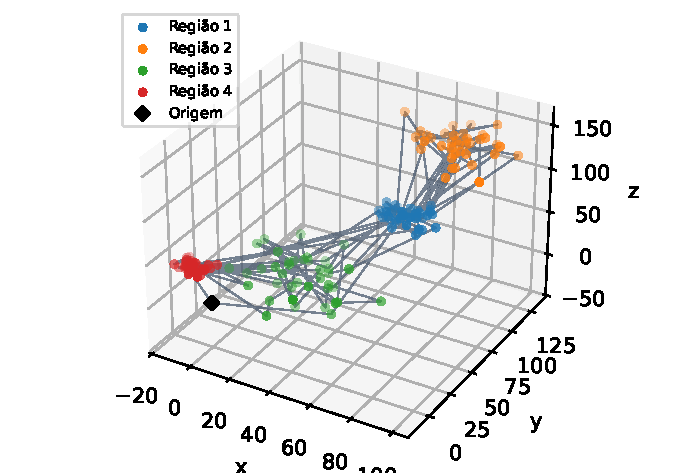
\includegraphics[width=.68\columnwidth]{rota.pdf}\caption{Melhor circuito encontrado. O marcador preto indica a origem.}\end{figure}
\subsection{Comparação em 50 dimensões}
\begin{table}[!ht]\centering\caption{Qualidade e tempo por rodada em 50 dimensões}
\scriptsize\setlength{\tabcolsep}{4pt}\begin{tabular}{lrrrr}\toprule
Método & $P$ & Melhor & Mediana & Tempo (s)\\
\midrule
GA-SBX & 20 & $161{,}145$ & $185{,}922$ & $0{,}136$\\
GA-SBX & 50 & $115{,}420$ & $174{,}014$ & $0{,}094$\\
GA-SBX & 100 & $141{,}252$ & $210{,}601$ & $0{,}065$\\
GA-SBX & 200 & $285{,}890$ & $367{,}748$ & $0{,}063$\\
LRS & --- & $0{,}022$ & $0{,}056$ & $0{,}173$\\
\bottomrule\end{tabular}\end{table}
O GA com 50 indivíduos apresentou a menor mediana entre os GAs e menor tempo médio que o GA com 20 indivíduos. As populações 100 e 200 terminaram mais rápido, mas com medianas piores. Sob orçamento fixo, elas renovaram a população menos vezes. A LRS obteve o menor custo final com memória de trabalho linear. A função é separável, o que favorece o ajuste de uma coordenada por vez. Nesta implementação, o tempo médio da LRS foi maior, em parte porque o GA avaliou lotes em NumPy.
\begin{figure}[!ht]\centering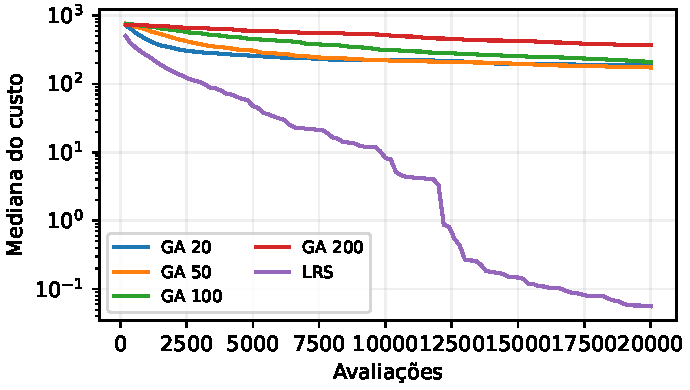
\includegraphics[width=.84\columnwidth]{convergencia.pdf}\caption{Mediana do melhor custo por orçamento de avaliações em 50 dimensões.}\end{figure}
